% Asset ID: AS1DifferentiationTIKZ-002
% Source: Chapter 12 Differentiation PDF pp.4-6 + CCEA AS1-DIFF-LO002
% Related lesson section: Core Theory 2-5
% Purpose: Show secant gradients approaching the tangent gradient as h tends to 0.

\documentclass[tikz,border=8pt]{standalone}
\usepackage{amsmath}
\usepackage{pgfplots}
\pgfplotsset{compat=1.18}

\begin{document}
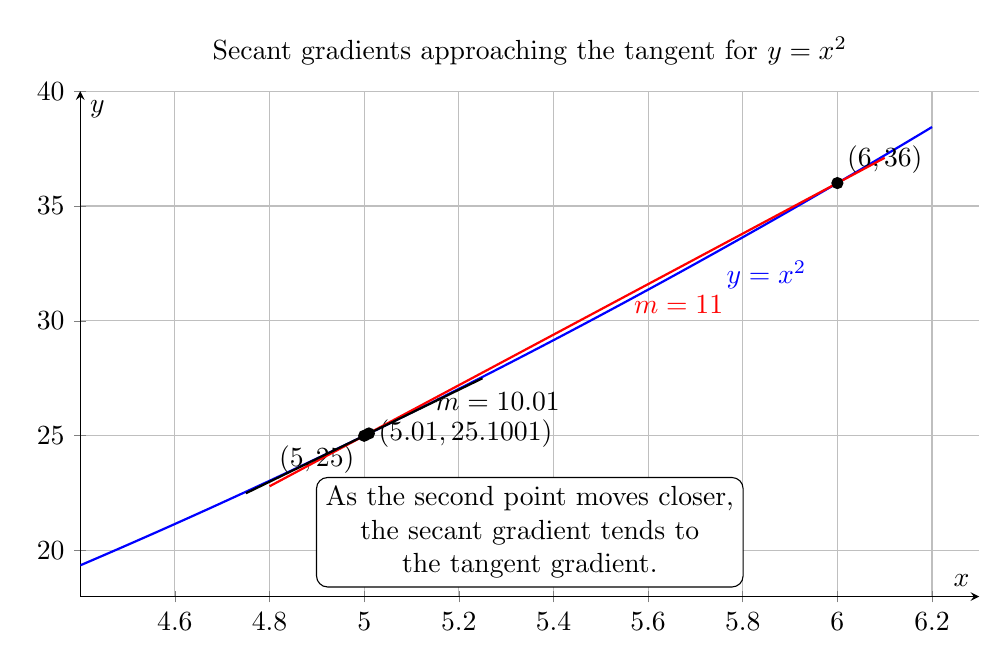
\begin{tikzpicture}
\begin{axis}[
    width=13cm,
    height=8cm,
    axis lines=middle,
    xmin=4.4, xmax=6.3,
    ymin=18, ymax=40,
    grid=both,
    xlabel={$x$},
    ylabel={$y$},
    title={Secant gradients approaching the tangent for $y=x^2$},
    samples=200,
    domain=4.4:6.2
]
\addplot[thick, blue] {x^2};
\node[blue] at (axis cs:5.85,32) {$y=x^2$};

\addplot[only marks, mark=*, black] coordinates {(5,25) (6,36) (5.01,25.1001)};
\node[anchor=north east] at (axis cs:5,25) {$(5,25)$};
\node[anchor=south west] at (axis cs:6,36) {$(6,36)$};
\node[anchor=west] at (axis cs:5.01,25.1001) {$(5.01,25.1001)$};

\addplot[red, thick, domain=4.8:6.1] {11*(x-5)+25};
\node[red, anchor=west] at (axis cs:5.55,30.7) {$m=11$};

\addplot[black, thick, domain=4.75:5.25] {10.01*(x-5)+25};
\node[black, anchor=west] at (axis cs:5.13,26.5) {$m=10.01$};

\node[fill=white, draw, rounded corners, align=center] at (axis cs:5.35,20.8)
{As the second point moves closer,\\the secant gradient tends to\\the tangent gradient.};

\end{axis}
\end{tikzpicture}
\end{document}
